%---------------------------------------------------------------------
\begin{frame}{Reminder last week}

    Three main ``legs'' of the ACA:
    \begin{enumerate}
        \item \newbold{Regulation} of the individual market
        \item An \newbold{individual mandate}
        \item Policies making insurance \newbold{more affordable}
    \end{enumerate}

    \vspace{3mm}

    Logic:
    \begin{itemize}
        \item Regulation alone risks adverse selection
        \item A mandate alone is regressive
        \item Subsidies make broad participation politically and financially feasible
    \end{itemize}

\end{frame}
%---------------------------------------------------------------------
\begin{frame}{A decrease of the number of uninsured}

   \begin{center}
    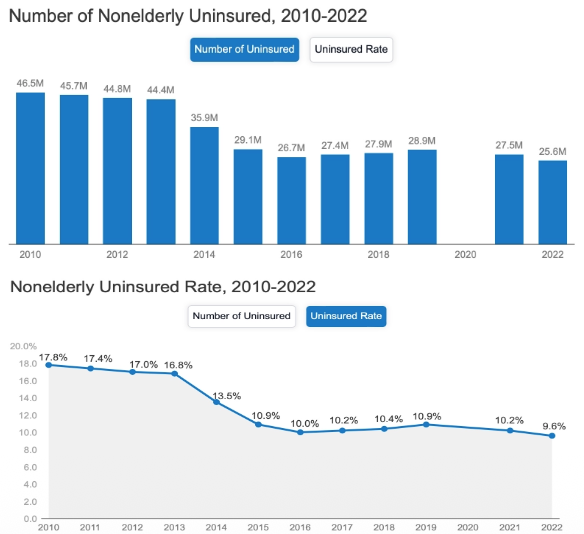
\includegraphics[width=0.5\textwidth]{input/uninsured_graphs.png}
    \end{center}
    \vspace{-3mm}
    {\tiny Source: \href{https://www.kff.org/uninsured/key-facts-about-the-uninsured-population/}{KFF website}.}

\end{frame}
%---------------------------------------------------------------------
\begin{frame}{Main coverage effect of the ACA}

    The uninsured rate for the non-elderly fell sharply after the ACA's main provisions took effect in 2014.

    \begin{itemize}
        \item 2014 uninsured rate: \newbold{13.9\%}
        \item 2015 uninsured rate: \newbold{10.9\%}
        \item Roughly \newbold{12.5 million} more people had coverage compared with 2013
    \end{itemize}

    \vspace{3mm}

    2014-2015: Medicaid enrollment increased by about \newbold{15 million}, and about \newbold{11 million} people purchased insurance on ACA marketplaces.\\
    \newbold{2025}: about 24 million people purchased insurance on the ACA marketplaces

\end{frame}
%---------------------------------------------------------------------
\begin{frame}{Where is the decrease in uninsured coming from?}

    \begin{center}
        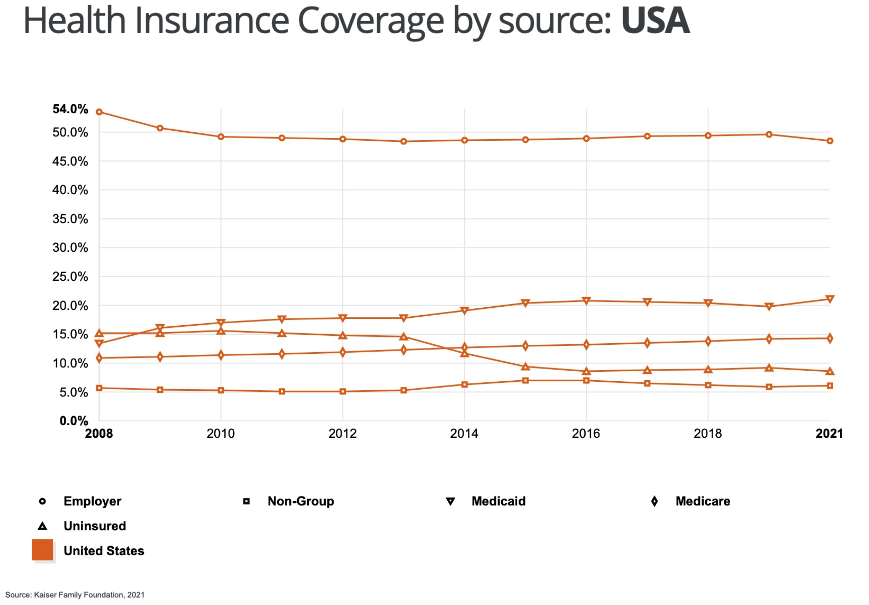
\includegraphics[width=0.8\textwidth]{input/KFF_sourcecoverage2021.png}
    \end{center}

\end{frame}
%---------------------------------------------------------------------
\begin{frame}{What drove the coverage gains?}

    Coverage gains seem to come mostly from:
    \begin{itemize}
        \item \newbold{Medicaid expansion}
        \item \newbold{Premium subsidies and marketplace regulation}
    \end{itemize}

    \vspace{3mm}

    The individual mandate appears to have played a \newbold{smaller role}.

    \vspace{3mm}

    There was also a \newbold{woodwork effect}:
    \begin{itemize}
        \item Publicity around the ACA encouraged some already-eligible people to enroll in Medicaid
    \end{itemize}

\end{frame}
%---------------------------------------------------------------------
\begin{frame}{Did employer insurance collapse?}

    One fear was that employers would drop coverage and send workers to the exchanges\\
    $\implies$ It did \newbold{not} happen on a large scale

    \begin{itemize}
        \item Employer-sponsored insurance remained the dominant source of coverage
        \item The share relying on employer plans was roughly unchanged
    \end{itemize}

    \vspace{3mm}

    So the ACA mainly expanded coverage without replacing the employer-based system.

\end{frame}
%---------------------------------------------------------------------
\begin{frame}{Takeaways: consequences of the ACA}

    The impact of the ACA
    \begin{enumerate}
        \item Decreased the share of uninsured by about half
        \item It did so without collapsing employer-sponsored insurance
        \item The Marketplace is relatively stable as of today
    \end{enumerate}
    \vspace{7mm}

    Even after the ACA, there remain about \newbold{25 million} people uninsured

\end{frame}
%---------------------------------------------------------------------
\begin{frame}{}
    \begin{center}
    \Large \textcolor{maroon}{Why are there still people who are uninsured?}
    \end{center}
\end{frame}
%---------------------------------------------------------------------
\begin{frame}{Who remained uninsured?}

    Who remains uninsured?
    \begin{itemize}
        \item Uninsurance is especially high among \newbold{young adults}
        \item Rates jump when public or dependent coverage ends
        \item Younger adults may be healthier and more willing to remain uninsured
    \end{itemize}

    \vspace{7mm}

    $\implies$ The healthiest part of the risk pool was still not fully participating

\end{frame}
%---------------------------------------------------------------------
\begin{frame}{Some fall through the cracks}

    There are still people not covered by the ACA
    \begin{itemize}
        \item People that are poor but not ``poor enough'' to get Medicaid in some states

        \begin{center}
            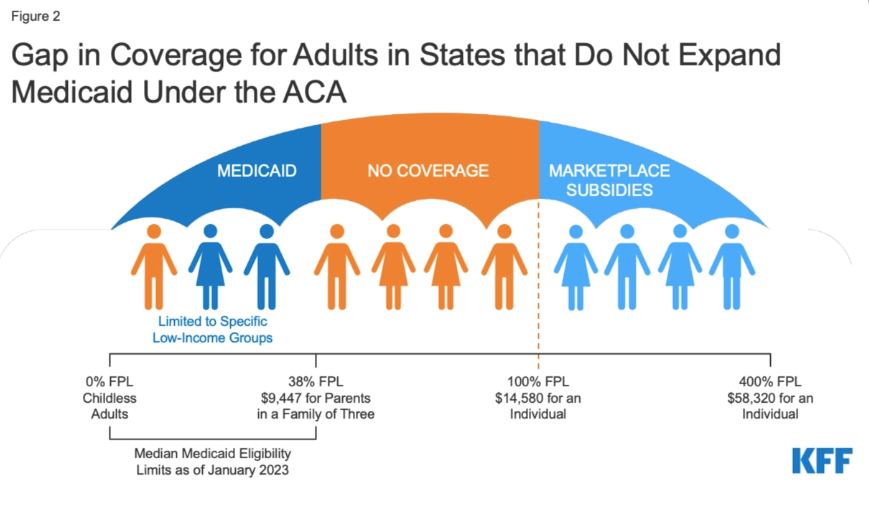
\includegraphics[width=0.5\textwidth]{input/Medicaid_gap.png}
        \end{center}
        \item Short-term uninsurance: when transition between plans or situations (loose job, gain job, etc.)
        \item Undocumented immigrants
    \end{itemize}

\end{frame}
%---------------------------------------------------------------------
\begin{frame}{Healthcare for the uninsured}

    Let's understand what happens when you don't have health insurance

    \vspace{7mm}

    If you show up at the hospital without health insurance, can they turn you away?\\
    \only<1>{{\color{white} No.}}\only<2>{\newbold{No!} \textit{(well, it depends on what care you need)}}

\end{frame}
%---------------------------------------------------------------------
\begin{frame}{EMTALA}

    \newbold{Emergency Medical Treatment and Labor Act (EMTALA)} is a U.S. federal law passed in 1986 that \textbf{requires hospitals to provide emergency care} regardless of a patient's ability to pay
    \begin{itemize}
        \item Enacted in response to the practice of ``patient dumping''
        \item Requires:
        \begin{enumerate}
            \item Medical screening examination to anyone seeking emergency care
            \item To stabilize the patient
            \item Appropriate transfer if needed (if stable or if benefits outweigh risks)
        \end{enumerate}
    \end{itemize}
    \vspace{3mm}

    %additional: covers all hospitals that accept medicare fudning, so almost all hospitals

    Note:
    \begin{itemize}
        \item Only emergency care
        \item Does not go beyond stabilization
        \item Does not mean the patient will not be charged
    \end{itemize}


\end{frame}
%---------------------------------------------------------------------
\begin{frame}{The ``Samaritan'' dilemma}

    Hospitals in the U.S. provide health care to the uninsured for several reasons
    \begin{itemize}
        \item EMTALA
        \item Non-profit status \textit{(more on this in two weeks)}
        \item Medical ethics
    \end{itemize}
    \vspace{5mm}

    \newbold{Uncompensated care}: the value of healthcare services provided by a hospital for which no payment is received from the patient or any third-party payer (charity care + bad debt)\\
    $\implies$ How would you compute it: charges versus costs?\\
    %Bad debt are payments that are never collected
    \pause
    \vspace{5mm}
    How much? $\sim$ \$50 billion each year (Garthwaite, Gross, and Notowidigdo 2018)
    \begin{itemize}
        \item That's about 70\% of all hospital profits
    \end{itemize}

\end{frame}
%---------------------------------------------------------------------
\begin{frame}{The ``Samaritan'' dilemma and incentives}

    Are people who remain uninsured taking advantage of this? \textit{Maybe, for some of them.}
    \begin{itemize}
        \item Remember the MA reform of 2006? That was part of the campaign for it\\
        \textit{``Why pay for something you can get for free?''}
        \item What does the research say?\\
        Some evidence for this: Mahoney (2015)\\
        $\implies$ Some people seem to be using bankruptcy as \textit{implicit} health insurance
    \end{itemize}
    \vspace{5mm}

    Is it the entire story? \textit{Probably not.}\\
    \vspace{5mm}

    Note: The Samaritan's dilemma is another rationale for government involvement in health insurance markets
    % In addition to adverse selection

\end{frame}
%---------------------------------------------------------------------
\begin{frame}{Very low willingness-to-pay for insurance for some people?}

    Could some people just have very low willingness-to-pay for insurance?
    \begin{itemize}
        \item Remember the Einav and Finkelstein framework:
        What if some people's willingness-to-pay is below their expected cost with insurance?
    \end{itemize}
    \vspace{5mm}

    What does the research say? \pause Some evidence for this.

\end{frame}
%---------------------------------------------------------------------
% \begin{frame}{Evidence in MA: Finkelstein, Hendren, Shepard (2019)}

% \begin{center}
%     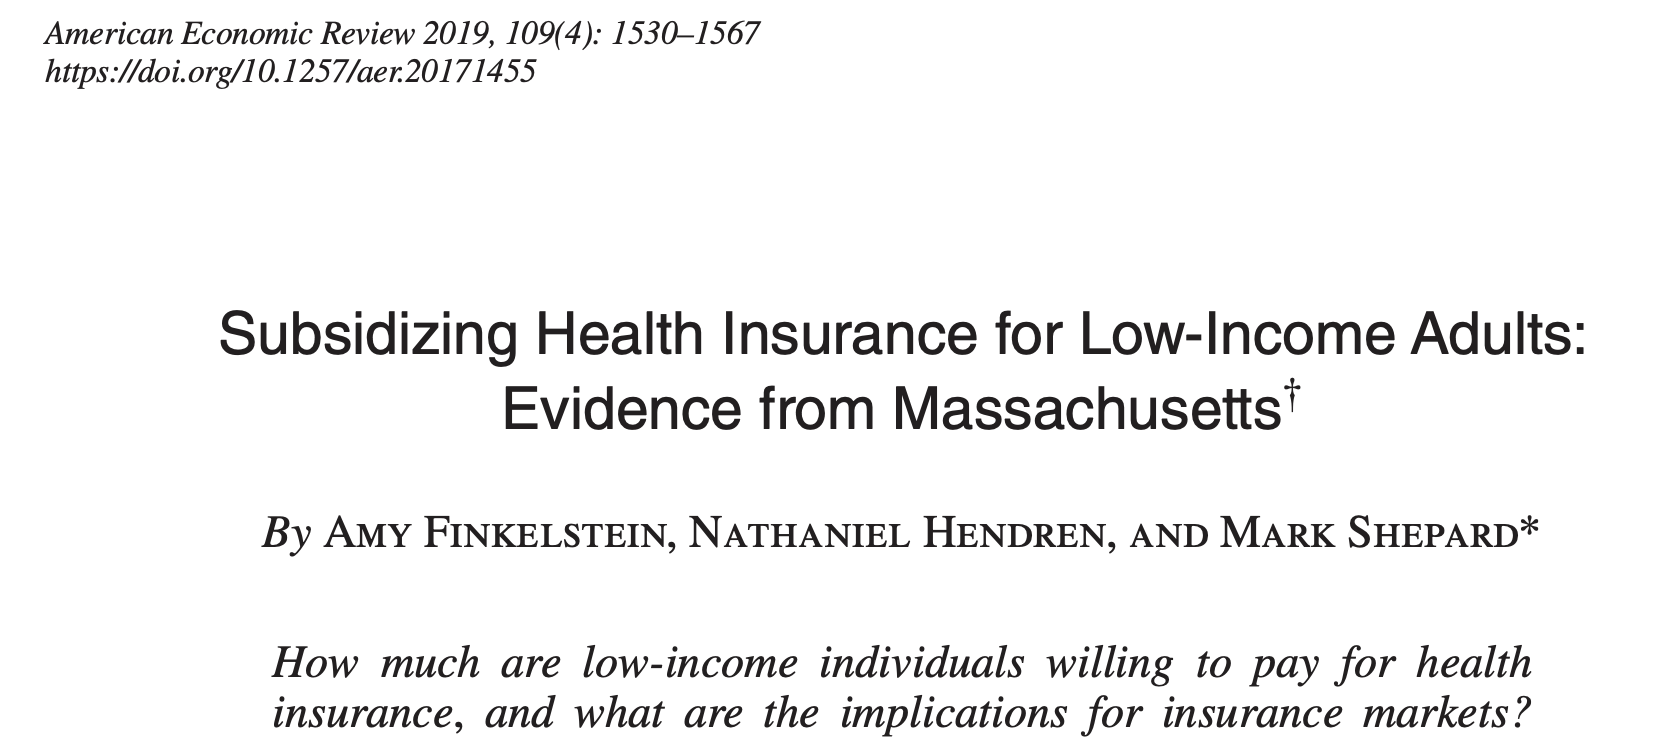
\includegraphics[width=0.8\textwidth]{input/FHS2019_front.png}
% \end{center}

% \end{frame}
% %---------------------------------------------------------------------
% \begin{frame}{Evidence in MA: Finkelstein, Hendren, Shepard (2019)}

%     \newbold{Setting}: Massachussetts insurance exchange\\
%     \vspace{5mm}

%     \newbold{Method}: use discontinuities in the subsidy schedule to estimate
%     \begin{itemize}
%         \item Cost of insurance for low-income adults (MC and AC)
%         \item Willingness to pay for insurance of low-income adults
%     \end{itemize}

% \end{frame}
% %---------------------------------------------------------------------
% \begin{frame}{Subsidy and premium discontinuities in 2011 in MA}

%     \begin{center}
%         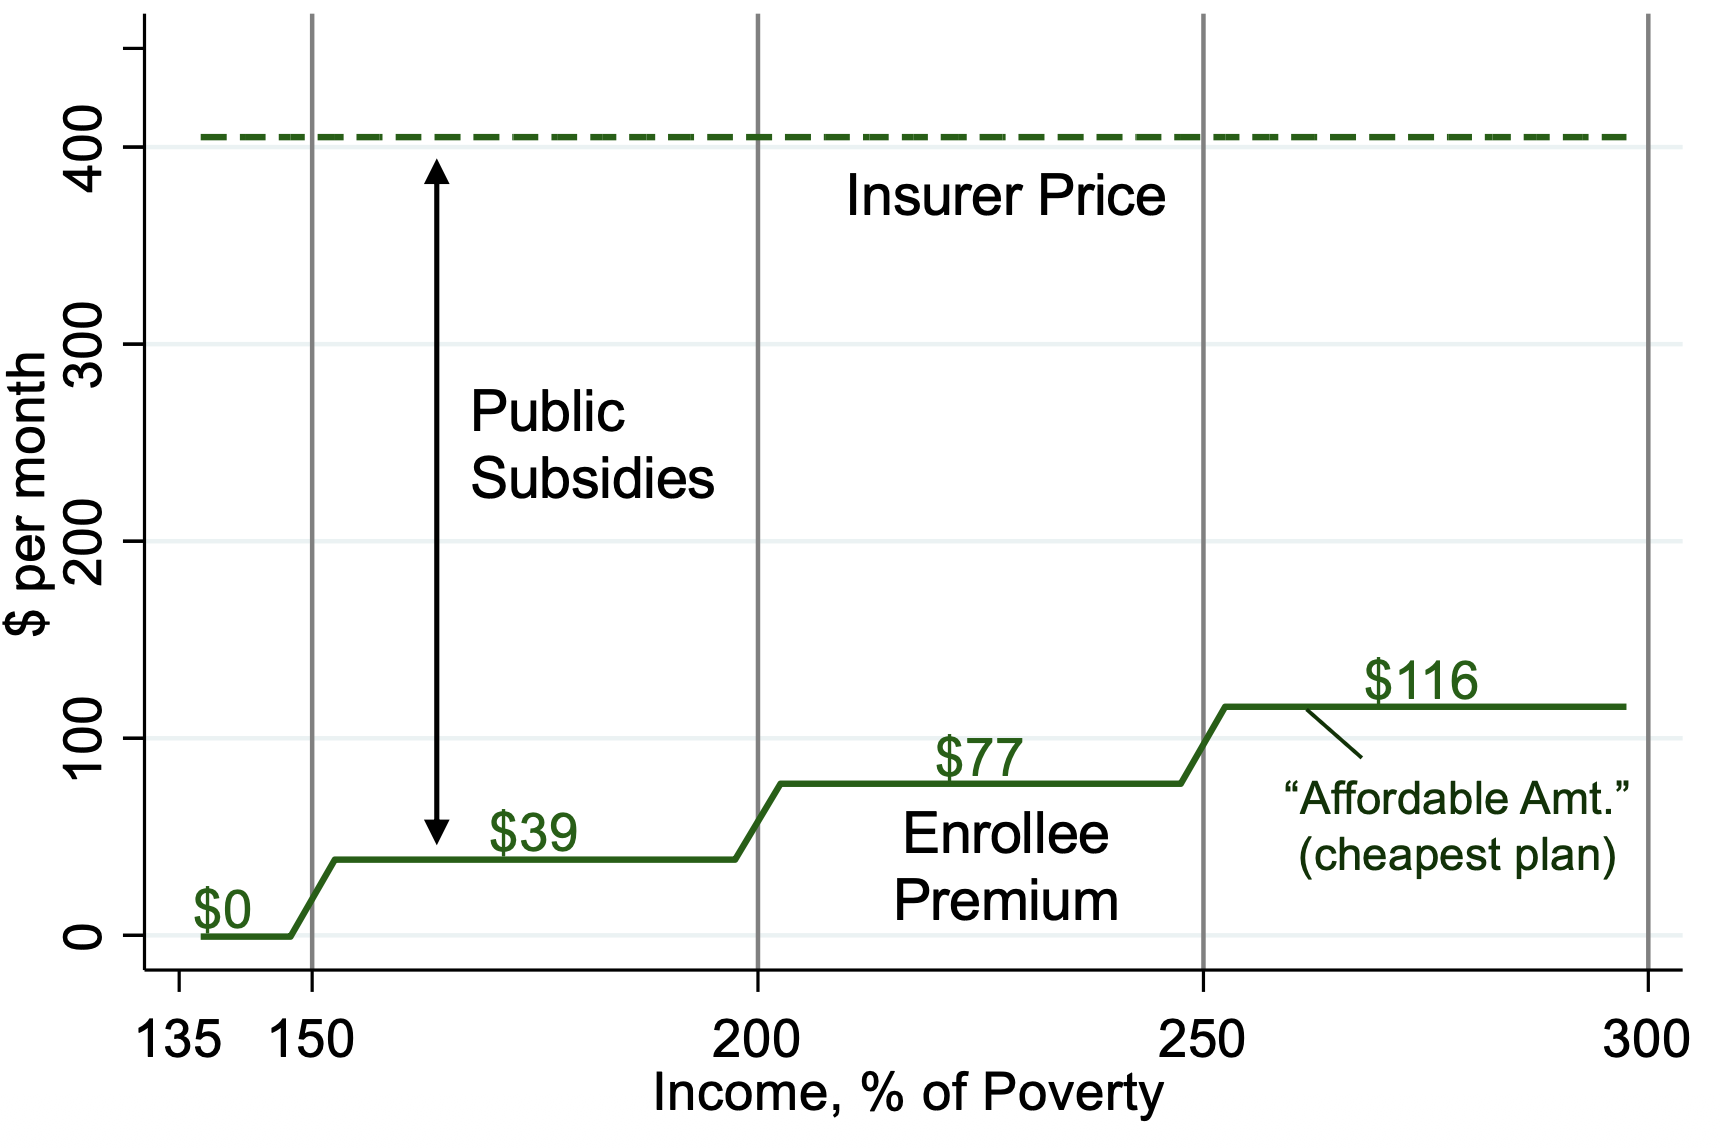
\includegraphics[width=0.8\textwidth]{input/FHS2029_fig2Mattslides.png}
%     \end{center}
%     % This comes from Matt's slides, that likely is a simplification fo figure 2

% \end{frame}
%---------------------------------------------------------------------
\begin{frame}{Cliff \textit{et al.} (2021)}

\newbold{Context}: Medicaid expansion in Michigan
\begin{itemize}
    \item Free for enrollees with income below the federal poverty level
    \item Premiums for enrollees with income above it was $\sim$\$3 per month
\end{itemize}
$\implies$ This is a very low price for insurance.
\pause 
\vspace{7mm}

\begin{enumerate}
    \item Did they find a large decrease in take-up of Medicaid for people above the poverty line?
    \item Were they high or low cost enrollees?
\end{enumerate}
\end{frame}
%---------------------------------------------------------------------
\begin{frame}{Cliff \textit{et al.} (2021)}

\begin{center}
    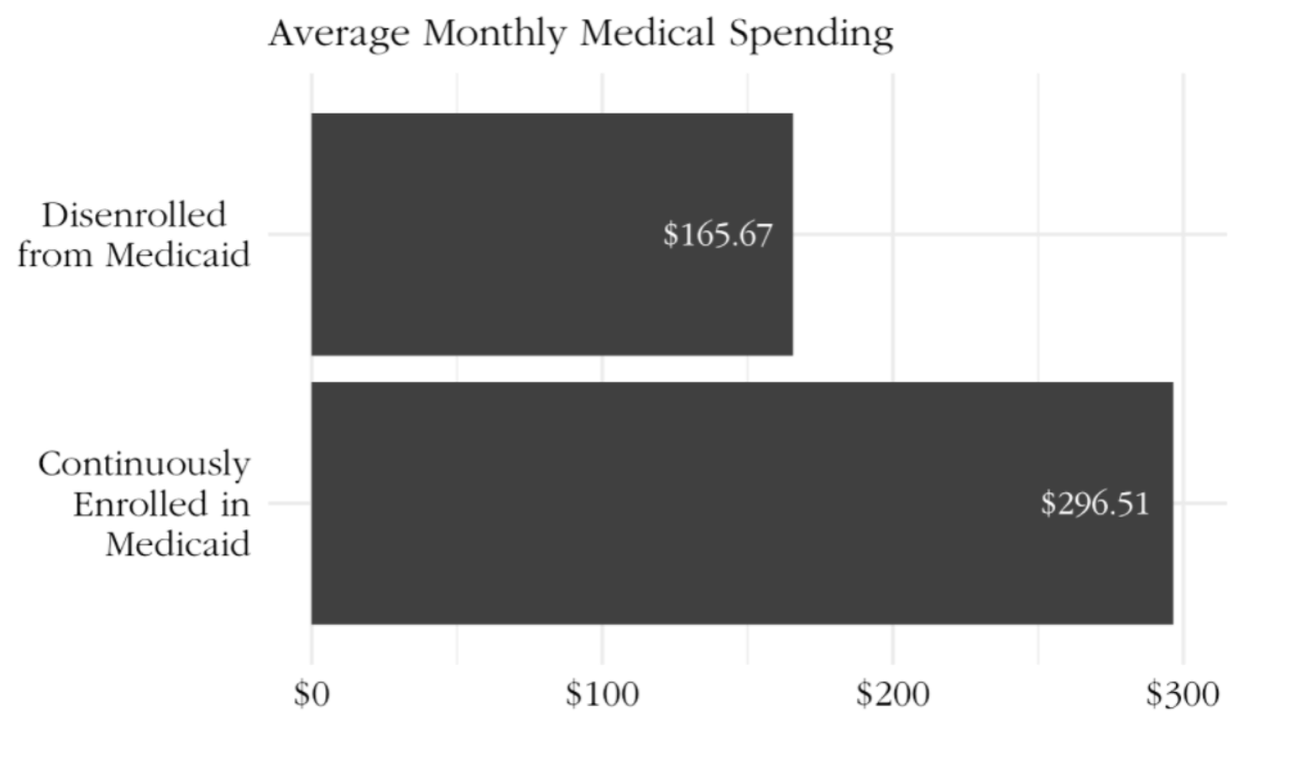
\includegraphics[width=0.8\textwidth]{input/Cliff_Notosbookfig1.png}
\end{center}
\end{frame}
%---------------------------------------------------------------------
\begin{frame}{Cliff \textit{et al.} (2021)}

\begin{center}
    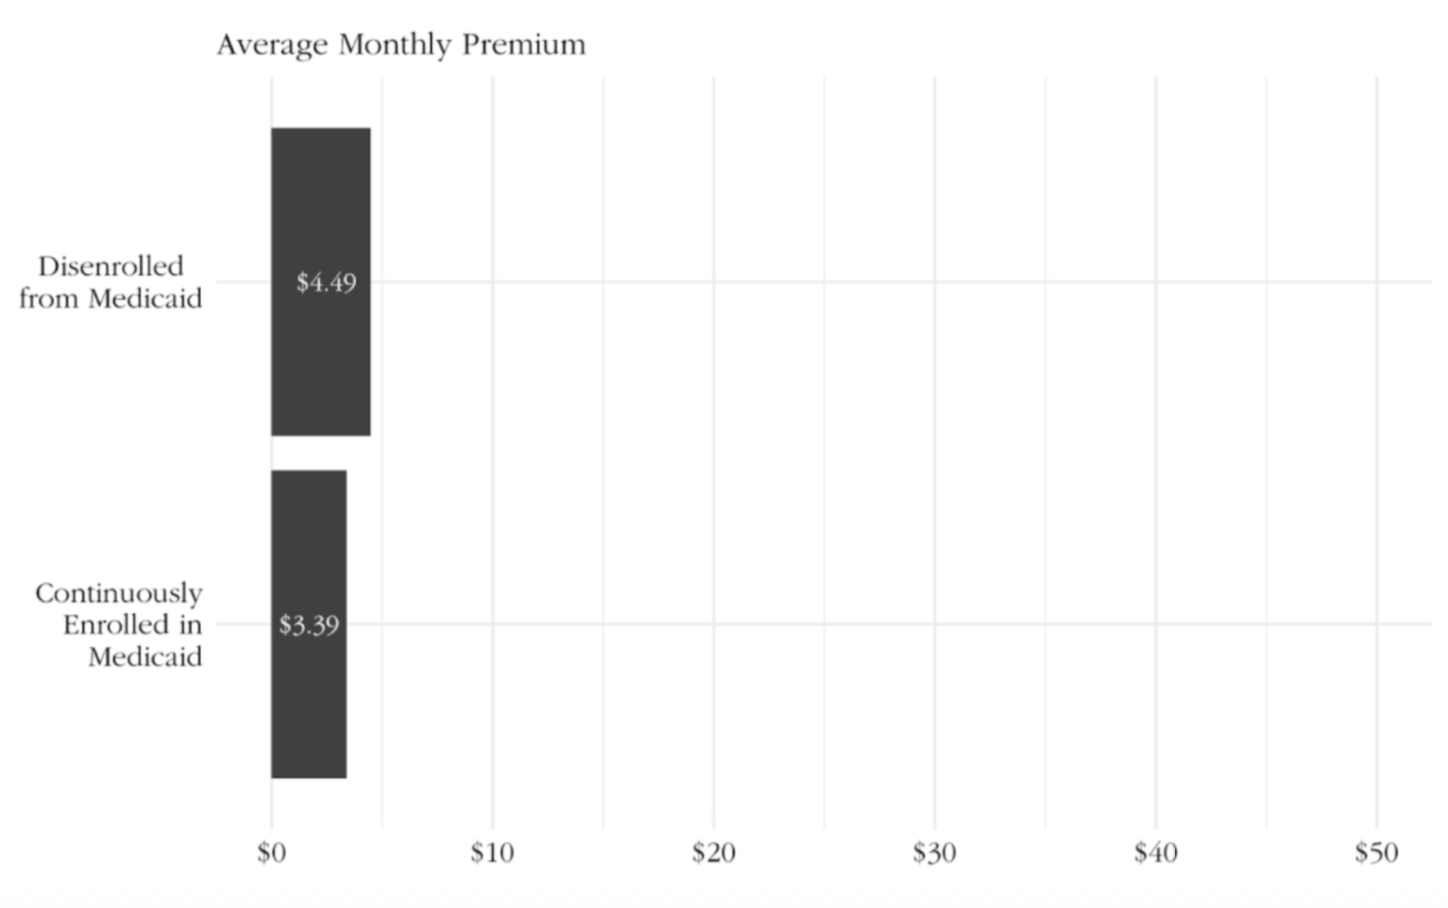
\includegraphics[width=0.8\textwidth]{input/Cliff_Notosbookfig2.png}
\end{center}
\end{frame}
%---------------------------------------------------------------------
\begin{frame}{WTP for insurance: what the research says}

    \begin{itemize}

        \item Cliff \textit{et al.} (2021) in Michigan\\
        \vspace{3mm}

        \item Finkelstein, Hendren, Shepard (2019) in Massachussetts:\\
        $\implies$ An increase in the premium per month of \$40 led to 25\% of people declining Medicaid coverage \\
        \vspace{3mm}

        \item Tebaldi (2021) in California\\
        $\implies$ The average amount people are willing to pay for health insurance on the exchange was far lower than the expected cost for the health insurer
    \end{itemize}

\end{frame}
%---------------------------------------------------------------------
\begin{frame}{Other explanations?}

    Getting health insurance may be costly for people beyond the monetary value
    \begin{itemize}
        \item \newbold{Search costs}: understanding the plans, gathering information, etc.\\
        $\implies$ This is time-consuming $\implies$ \textit{costly} for people
        \item \newbold{Lack of information}: people may not know and understand the regulation, options available, etc.\\
        \textit{Remember the IRS letters?}
        %THey may also not understand it
    \end{itemize}
\end{frame}
%---------------------------------------------------------------------
\begin{frame}{Who pays for the uninsured?}

    Imagine your are the CEO of a hospital.
    Your state decided to increase the threshold for Medicaid eligibility,
    so \textbf{less} people are now eligible for Medicaid and more people end up being uninsured.\\
    $\implies$ You will have more uncompensated care to provide.\\
    How would you adjust prices for the insured patients?

\end{frame}
%---------------------------------------------------------------------
\begin{frame}{Who pays for the uninsured?}

    How would you adjust prices for the insured patients?
    \only<1>{
    \begin{itemize}
        \item You may be tempted to \textit{increase} prices for the insured patients to compensate for the increase in uncompensated care (cost-shifting hypothesis)...
    \end{itemize}
    \vspace{35mm}
    }
    \only<2>{
    \begin{itemize}
        \item You may be tempted to \textit{increase} prices for the insured patients to compensate for the increase in uncompensated care (cost-shifting hypothesis)...
        \item ... but you may also be worried about losing insured patients by increasing prices.
        Instead, it may actually better to \textit{decrease} prices for the insured patients to attract more of them and compensate for the increase in uncompensated care.
    \end{itemize}
        \vspace{8mm}
    }
    \only<3>{
    \begin{itemize}
        \item You may be tempted to \textit{increase} prices for the insured patients to compensate for the increase in uncompensated care (cost-shifting hypothesis)...
        \item ... but you may also be worried about losing insured patients by increasing prices.\\
        Instead, it may actually better to \textit{decrease} prices for the insured patients to attract more of them and compensate for the increase in uncompensated care.
    \end{itemize}
    $\implies$ What do hospitals do then?
    \textit{Let's look at the research!}
    }    

\end{frame}
%---------------------------------------------------------------------
\begin{frame}{Garthwaite, Gross and Notowidigdo (2018)}

\begin{center}
    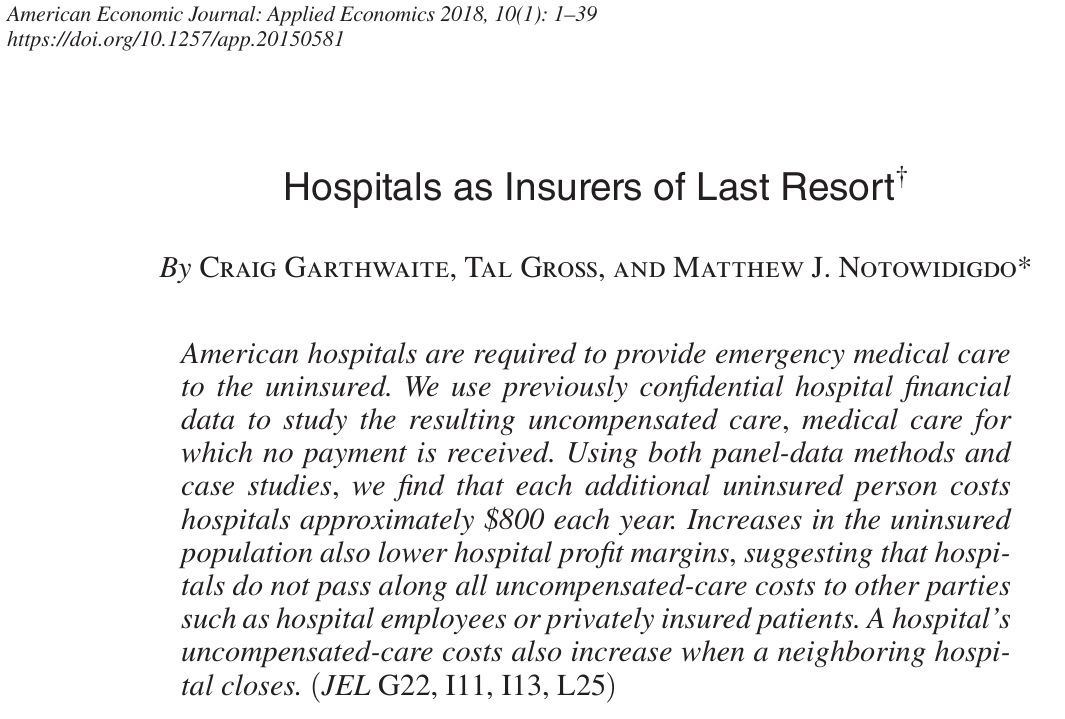
\includegraphics[width=0.75\textwidth]{input/GGN2018_front.png}
\end{center}    
\end{frame}
%---------------------------------------------------------------------
\begin{frame}{Garthwaite, Gross and Notowidigdo (2018)}

Approaches
\begin{itemize}
    \item Previously confidential data from the American Hospital Association (AHA) on hospital-level finances 1984-2011
    \item Disenrollment reforms in 2005 in Tennessee and Missouri
\end{itemize}
\vspace{3mm}

Main findings: 
\begin{itemize}
    \item Each newly uninsured person leads to nearly \$800 in uncompensated-care costs for hospital
    \item Increases in uninsured population \textit{decrease} hospitals' profit margins
\end{itemize}
$\implies$ Evidence against the cost-shifting hypothesis

\end{frame}
%---------------------------------------------------------------------
\begin{frame}{Cross-sectional evidence}

\begin{center}
    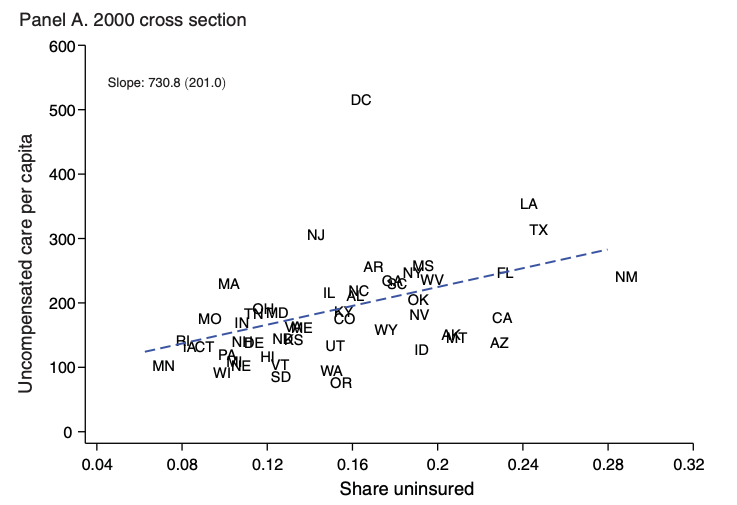
\includegraphics[width=0.7\textwidth]{input/GGN2018_fig1a.png}
\end{center}

\end{frame}
%---------------------------------------------------------------------
\begin{frame}{Panel evidence}

\begin{center}
    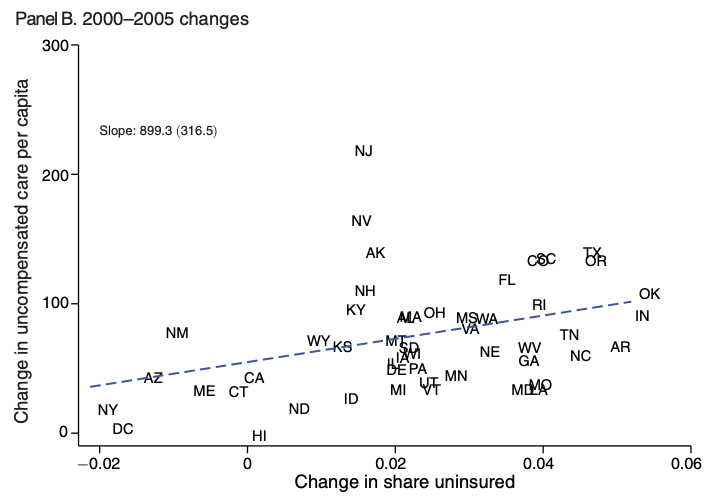
\includegraphics[width=0.7\textwidth]{input/GGN2018_fig1b.png}
\end{center}

% Issues: reverse causality. More charity ==> more insurers
% Otehr issue: unobserved counfounders, like recession spreading to some regions more than others.

\end{frame}
%---------------------------------------------------------------------
\begin{frame}{Tennessee: TennCare cuts}

\begin{center}
    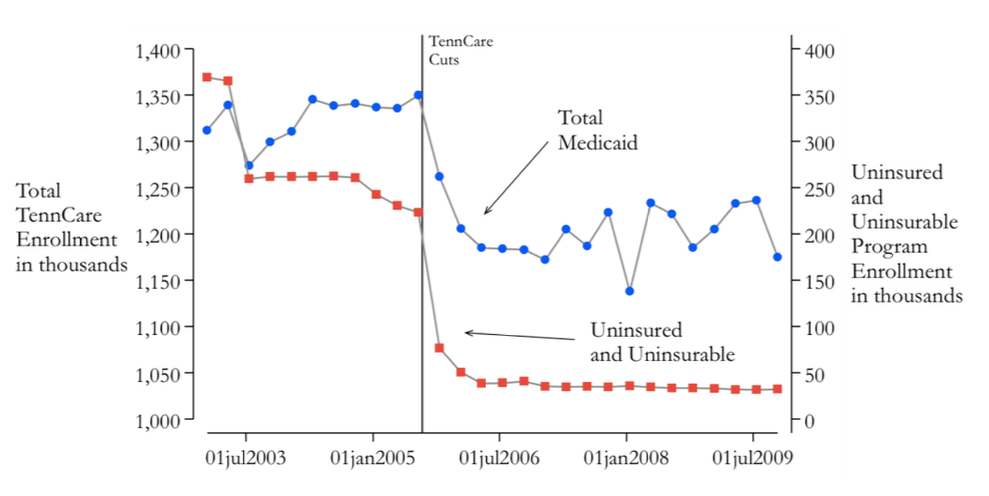
\includegraphics[width=0.95\textwidth]{input/GGN2018_TNdisenrollmentslides.png}
\end{center}

\end{frame}
%---------------------------------------------------------------------
\begin{frame}{Tennessee: TennCare cuts impact on cost}

    Difference: Tennessee versus other Southern states
\begin{center}
    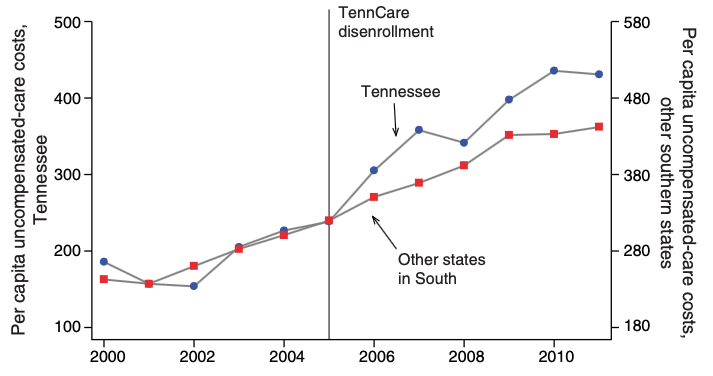
\includegraphics[width=0.8\textwidth]{input/GGN2018_fig3.png}
\end{center}

% What if shock in TN that prompted the policy change? ==> Within TN

\end{frame}
%---------------------------------------------------------------------
\begin{frame}{Tennessee: TennCare cuts impact on cost}

    Difference: Within Tennessee, regions more or less impacted by TennCare disenrollment
\begin{center}
    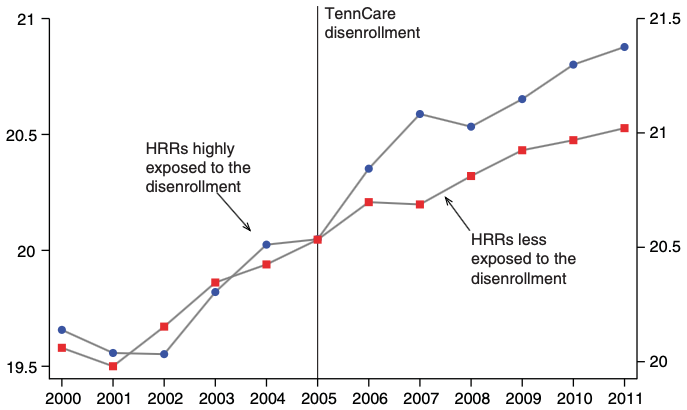
\includegraphics[width=0.7\textwidth]{input/GGN2018_fig4.png}
\end{center}

\end{frame}
%---------------------------------------------------------------------
\begin{frame}{Garthwaite, Gross and Notowidigdo (2018) - conlusion}

Main findings: 
\begin{itemize}
    \item Each newly uninsured person leads to nearly \$800 in uncompensated-care costs for hospital
    \item Increases in uninsured population \textit{decrease} hospitals' profit margins
\end{itemize}
$\implies$ Evidence \newbold{against} the \newbold{cost-shifting} hypothesis\\
\vspace{5mm}

\textit{They have more results in the paper that we will explore in two weeks when talking about hospitals.}

\end{frame}
%---------------------------------------------------------------------
\begin{frame}{Conclusion}

Consequences of the ACA:
\begin{itemize}
    \item Decrease in the number of uninsured by about half
    \item No collapse of employer-sponsored insurance
    \item The Marketplace is relatively stable as of today
\end{itemize}
\vspace{2mm}

However, still about 25 million people uninsured after the ACA. Why?
\begin{itemize}
    \item Samaritan's dilemma: another argument for government intervention in health insurance markets
    \item Some people may have very low willingness-to-pay for insurance
    \item Behavioral explanations: search costs and lack of information
\end{itemize}
\vspace{2mm}

Who pays for the uninsured? Evidence that hospitals are bearing (some of) this cost.

\end{frame}
%---------------------------------------------------------------------
\begin{frame}{}
    \begin{center}
    \Large \textcolor{maroon}{Wrapping up}
    \end{center}
\end{frame}
%---------------------------------------------------------------------
\begin{frame}{To next class}
\begin{itemize}
    \item \newbold{Midterm 2}: \newbold{Thursday April 2nd} in class
    \begin{itemize}
        \item Bring \newbold{BU ID} and \newbold{calculator}
        \item Closed book, closed notes
        \item Format: part 1 TFU questions, part 2 quantitative exercises
        \item Covers material from \textbf{week 6 to week 9 included}
    \end{itemize}
    \vspace{5mm}

    \item Program for next class
    \begin{itemize}
        \item Review session on Tuesday
    \end{itemize}
\end{itemize}
\end{frame}
%---------------------------------------------------------------------


% Uninsured types: https://www.kff.org/uninsured/health-policy-101-the-uninsured-population-and-health-coverage/?entry=table-of-contents-who-is-uninsured-in-the-united-states
% Other interesting reading on the uninsured: https://www.kff.org/wp-content/uploads/2013/01/8246.pdf